\documentclass{beamer}

\usetheme{Luebeck}
\usecolortheme{dove}

\usepackage{tikz}
\usetikzlibrary{arrows,automata} 

\usepackage{listings}

\usepackage{cite} 
\usepackage{natbib} %citep and citet
\def\newblock{\hskip .11em plus .33em minus .07em}
\renewcommand{\bibsection}{\subsubsection*{\bibname } }

\usepackage{amsmath}
\DeclareMathOperator*{\bigplus}{\mbox{\huge +}}

\begin{document}
\title{Constructive Formalization of Regular Languages}  
\author[Jan-Oliver Kaiser]{Jan-Oliver Kaiser \\{\small Advisors: Christian Doczkal, Gert Smolka }\\{\small Supervisor: Gert Smolka}}

\date{\today} 


\begin{frame}
    \titlepage
\end{frame}

\begin{frame}
    \tableofcontents
\end{frame}


\section*{Recap}
\begin{frame}
    \textbf{Definitions:} \\

    \begin{itemize}
        \item 
            We use extended regular Expressions (RE):
            \[    
                r, s ::= \emptyset \, | \, \varepsilon \, | \,  a \, | \, rs \, | \,  r \,  + \, s \, | \, r \, \& \, s \, |\, r^* \, | \, \neg r
            \]
            \[
            \mbox{\textbf{Def.:} }  \bigplus_{x \in X} r_x := r_{x_0} + ... + r_{x_{|X|-1}}
            \]

        \item 
            Our Finite Automata (FA) are
            \[
                (\Sigma, Q, q_0, F, \delta)
            \]
            (The transition relation $\delta$ of deterministic FA is total).
    \end{itemize}
\end{frame}

\section{Goal}
\subsection*{Current Goal}
\begin{frame}

    \textbf{Goal:}

    Find simple proofs for the decidability of regular expression equivalence and the Myhill-Nerode theorem.\\

    \textbf{Roadmap:}

    \begin{enumerate}
        \item RE $\Rightarrow$ FA (\textbf{DONE})
        \item Emptiness test on FA (\textbf{Easy})
        \item RE equivalence (\textbf{Follows from 1 and 2})
        \item FA $\Rightarrow$ RE (\textbf{Work in progress})
        \item Myhill-Nerode
    \end{enumerate}

\end{frame}

\section*{Finite automata to regular expressions}
\subsection*{Difficulty}
\begin{frame}

    \large{\textbf{Finite automata to regular expressions}}

    \begin{itemize}
        \item
            Converting REs to FAs is straight-forward and there is really only one algorithm (with slight variations): \\
            We mirror the constructors of RE in operations on FAs.

            \pause

        \item
            Converting FAs to REs is complicated and there are at least three algorithms found in textbooks.
    \end{itemize}

    \pause

    {\centering 
        \textbf{Why is that?}

    }

\end{frame}

\begin{frame}
    \textbf{My intuition:} 
    \begin{itemize}
        \item
            Converting REs to FAs is done by structural recursion on a \textbf{tree}. The result is a \textbf{flat structure}.

            \pause

        \item
            Converting FAs to REs \textbf{can not be done} by structural recursion.
            There is \textbf{no recursive structure} in FAs. \\
            But somehow we need to construct a \textbf{tree} of REs.
    \end{itemize}



\end{frame}

\subsection*{Overview}
\begin{frame}

    \textbf{Three methods (+ variations):}

    \begin{enumerate}
        \item Transitive Closure (Kleene \cite{KleeneNets})
        \item State Removal (Du, Ko \cite{DuKo}, simplified in Linz \cite{DBLP:books/daglib/0019552})
        \item Brzozowski Algebraic Method (Brzozowski \cite{DBLP:journals/jacm/Brzozowski64})
    \end{enumerate}

\end{frame}


\section{State Removal}
\subsection*{Approach}
\begin{frame}
    \textbf{State Removal}    

    \textbf{Given}: NFA $A$ = $(\Sigma, Q, q_0, F, \delta)$.

    \textbf{New concept}: Automata that have transitions labeled by RE.

    \textbf{Idea}: Remove states until there are two or less states remaining. Update the remaining states' transitions by incorporating the "lost" paths.


\end{frame}

\subsection*{Algorithm}
\begin{frame}
    \textbf{Remove $q$ from}\\

    \begin{figure}
        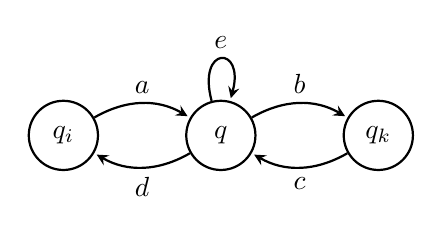
\begin{tikzpicture}[shorten >=1pt,node distance=2cm,>=stealth,thick]
            \node[state] (1) {$q_i$};
            \node[state] (2) [right of=1] {$q$};
            \node[state] (3) [right of=2] {$q_k$};
            \draw [->] (1) to[bend left] node[auto] {$a$} (2);
            \draw [->] (2) to[bend left] node[auto] {$b$} (3);
            \draw [->] (2) to[loop above] node[auto] {$e$} (2);
            \draw [->] (3) to[bend left] node[auto] {$c$} (2);
            \draw [->] (2) to[bend left] node[auto] {$d$} (1);
        \end{tikzpicture}
        \\
    \end{figure}

    \pause

    \textbf{to get}\\

    \begin{figure}
        \begin{tikzpicture}[shorten >=1pt,node distance=2cm,>=stealth,thick]
            \node[state] (1) {$q_i$};
            \node[state] (3) [right of=2] {$q_k$};
            \draw [->] (1) to[bend left] node[auto] {$ae^*b$} (3);
            \draw [->] (1) to[loop above] node[auto] {$ae^*d$} (1);
            \draw [->] (3) to[bend left] node[auto] {$ce^*d$} (1);
            \draw [->] (3) to[loop above] node[auto] {$ce^*b$} (3);
        \end{tikzpicture}
        \\
    \end{figure}

\end{frame}

\begin{frame}
    \textbf{Repeat until $A$ is of this form:}

    \begin{figure}
        \begin{tikzpicture}[shorten >=1pt,node distance=2cm,>=stealth,thick]
            \node[state] (1) {$q_1$};
            \node[state] (3) [right of=2, accepting] {$q_f$};
            \draw [->] (1) to[bend left] node[auto] {$r_2$} (3);
            \draw [->] (1) to[loop above] node[auto] {$r_1$} (1);
            \draw [->] (3) to[bend left] node[auto] {$r_3$} (1);
            \draw [->] (3) to[loop above] node[auto] {$r_4$} (3);
        \end{tikzpicture}
        \\
        $\Rightarrow \mathcal{L}(A) = \mathcal{L}(r_1^* r_2 (r_4 + r_3 r_1^* r_2)^*)$
    \end{figure}


\end{frame}

\subsection*{Caveats}
\begin{frame}
    \textbf{Caveats} \\
    \begin{itemize}
        \item
            It looks like we only need to update two edges. \\
            \pause
            In reality, there can be $|Q|-1$ states connected to $q$.
            \pause

            \begin{figure}
                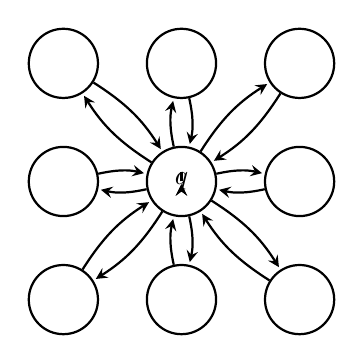
\begin{tikzpicture}[shorten >=1pt,node distance=1.5cm,>=stealth,thick,minimum size=1cm]
                    \node[state] (q11) {};
                    \node[state] (q12) [right of = q11] {};
                    \node[state] (q13) [right of = q12] {};
                    \node[state] (q21) [below of = q11] {};
                    \node[state] (q22) [right of = q21] {$q$};
                    \node[state] (q23) [right of = q22] {};
                    \node[state] (q31) [below of = q21] {};
                    \node[state] (q32) [right of = q31] {};
                    \node[state] (q33) [right of = q32] {};

                    \draw [->] (q11) to[bend left=12.5] node[auto] {} (q22);
                    \draw [->] (q22) to[bend left=12.5] node[auto] {} (q11);

                    \draw [->] (q12) to[bend left=12.5] node[auto] {} (q22);
                    \draw [->] (q22) to[bend left=12.5] node[auto] {} (q12);

                    \draw [->] (q13) to[bend left=12.5] node[auto] {} (q22);
                    \draw [->] (q22) to[bend left=12.5] node[auto] {} (q13);

                    \draw [->] (q21) to[bend left=12.5] node[auto] {} (q22);
                    \draw [->] (q22) to[bend left=12.5] node[auto] {} (q21);

                    \draw [->] (q22) to[bend left=12.5] node[auto] {} (q22);
                    \draw [->] (q22) to[bend left=12.5] node[auto] {} (q22);

                    \draw [->] (q23) to[bend left=12.5] node[auto] {} (q22);
                    \draw [->] (q22) to[bend left=12.5] node[auto] {} (q23);

                    \draw [->] (q31) to[bend left=12.5] node[auto] {} (q22);
                    \draw [->] (q22) to[bend left=12.5] node[auto] {} (q31);

                    \draw [->] (q32) to[bend left=12.5] node[auto] {} (q22);
                    \draw [->] (q22) to[bend left=12.5] node[auto] {} (q32);

                    \draw [->] (q33) to[bend left=12.5] node[auto] {} (q22);
                    \draw [->] (q22) to[bend left=12.5] node[auto] {} (q33);


                \end{tikzpicture}
            \end{figure}


    \end{itemize}
\end{frame}

\begin{frame}
    \textbf{Caveats} \\
    \begin{itemize}
        \item
            It looks like we only need to update two edges. \\
            In reality, there can be $|Q|-1$ states connected to $q$.
        \item
            What about final states?\\
            \pause
            \begin{enumerate}
                \item
                    Introduce a new final state without any outgoing edges.
                \item
                    Introduce $\varepsilon$ transitions from all other final states to the final new state.
                \item
                    Make all other states non-final.
                \item
                    Never remove the new final state.
            \end{enumerate}
    \end{itemize}
\end{frame}

\subsection*{Properties}
\begin{frame}
    \textbf{Formalization:} \\
    \begin{itemize}
        \item
            Requires a new kind of finite automaton that has RE transitions.
        \item
            Lots of details to consider.
        \item
            Induction on the number of states.
    \end{itemize}
\end{frame}

\section{Brzozowski Algebraic Method}
\subsection*{Approach}
\begin{frame}
    \textbf{Brzozowski Algebraic Method}

    \textbf{Given}: FA $A$ = $(\Sigma, Q, q_0, F, \delta)$.\\
    \textbf{Idea}: Retrieve a RE for FA by solving a system of equations determined by $\delta$.

\end{frame}

\subsection*{Algorithm}
\begin{frame}
    \textbf{Construct system of equations}:

    \begin{equation*}
        \begin{array}{lcll} 
            r_0 & = & 
            \displaystyle\sum\limits_{
                \substack{a \in \Sigma \\ 0 \leq i < |Q|} 
            }
            \{ \, a \, r_i \, |  \, (q_0, a, q_i) \in \delta \} 
            &
            (+ \, \varepsilon \mbox{ if } r_0 \in F)
            \\ 
            \vdots &  = & \vdots \\
         r_{|Q|-1} & = & 
            \displaystyle\sum\limits_{
                \substack{a \in \Sigma \\ 0 \leq i < |Q|} 
            }
            \{ \, a \, r_i \, |  \, (q_{|Q|-1}, a, q_i) \in \delta \} 
            &
            (+ \, \varepsilon \mbox{ if } r_{|Q|-1} \in F)
            \\ 
        \end{array}
    \end{equation*}
    $\, \Rightarrow \mathcal{L}(A) = \mathcal{L}(r_0)$
\end{frame}

\begin{frame}
    Solve the system by substitution and \textbf{Arden's Lemma} which states that for all regular languages X, Y and Z the equation
    \begin{equation}
        \begin{array}{lcl}
            X = YX + Z
        \end{array}
    \end{equation}

    has the unique solution

    \begin{equation}
        \begin{array}{lcl}
            X = Y^*Z
        \end{array}
    \end{equation}
\end{frame}

\subsection*{Properties}
\begin{frame}
    \textbf{Formalization:} \\
    \begin{itemize}
        \item
            Requires a formalization of these equations and operations on them. 
        \item
            We would need to prove Arden's Lemma.
        \item
            We would also need to prove that Arden's Lemma (and substitution) is enough to solve these systems of equations.
    \end{itemize} 
\end{frame}

\section{Transitive Closure}
\subsection*{Approach}
\begin{frame}

    \large{\textbf{Transitive Closure}} \\

    \textbf{Given}: FA $A$ = $(\Sigma, Q, q_0, F, \delta)$.

    \textbf{Idea}: Construct regexps $r_f$ for all final states $f \in F$ s.t. \\$r_f$ matches all words which A accepts with final state $f$. \\

    \[
        \, \Rightarrow \mathcal{L}(A) = \mathcal{L}(\bigplus\limits_{f \in F} r_f)
    \]

    \vspace{5 mm}

    \textbf{How do we construct $r_f$?} 

\end{frame}

\subsection*{Algorithm}
\begin{frame}

    We generalize the idea of $r_f$ to $R^k_{i j}$ which matches all words which lead from state $i$ to $j$ while passing only through states with index smaller than $k$.

    \begin{enumerate}
        \item 
            Merge multiple edges between states to one unified edge.
        \item
            Construct regexp $R^k_{i j}$ recursively:

            \begin{description}

                \item[$R^0_{i j}$]
                    $ := \begin{cases} 
                        r & \mbox{if } i \neq j \wedge i \mbox{ has edge } r \mbox{ to j}  \\
          \varepsilon + r & \mbox{if } i = j \wedge i \mbox{ has edge } r \mbox{ to j}  \\
                \emptyset & \mbox{otherwise}
                    \end{cases}
                    $ 

                \item[$R^k_{i j}$]
                    $ := R^{k-1}_{i k} R^{k-1}_{k k} R^{k-1}_{k j} + R^{k-1}_{i j}$

            \end{description}

    \end{enumerate}

    \[ 
        \Rightarrow \mathcal{L}(A) = \mathcal{L}(\bigplus_{f \in F} r_f) = \mathcal{L}(\bigplus_{f \in F} R^{|Q|}_{0 f}) 
    \]

\end{frame}

\subsection*{Properties}
\begin{frame}
    \textbf{Formalization:} \\
    \begin{itemize}
        \item
            Easier than the other methods.\\
        \item
            The recursive definition translates quite well.\\
        \item
            The details are quite challenging.
    \end{itemize} 

    \pause

    {\centering 
        \textbf{This appears to be the simplest to formalize.}

    }
\end{frame}

\section{Our Approach}
\subsection*{Definitions}
\begin{frame}
    \textbf{Our Approach:} \\

    There are different ways of formalizing $R^k_{i j}$ itself, especially its parameters. Most practical so far: \\
    $k$ is of type nat, $i$ and $j$ are ordinals from $[0..|Q|-1]$.\\
    \pause
    This gives us easy recursion and matching on $k$.\\
    \pause
    \textbf{But} we have to use $min \, k \, (|Q|-1)$ to map k to the corresponding ordinal (and then to a state).

\end{frame}

\begin{frame}
    To get a FA counterpart to $R^k_{i j}$, we introduce $A^k_{i j}$ s.t.
    \[
        \mathcal{L}(A^k_{i j}) = \mathcal{L}(R^k_{i j}).
    \]
    $A^k_{i j}$ is similar to A. It has one additional state, which has all incoming edges of state $j$ and no outgoing edges. It only leaves states that are $i$ or  $<k$. It only enters states less than $<k$ or the new state.
    \\
    We can then show that  
    \[
        \mathcal{L}(\bigcup_{f \in F} A^{|Q|}_{q_0 f}) = \mathcal{L}(A).
    \]
\end{frame}

\subsection*{Lemmas}
\begin{frame}
    \textbf{Lemmas:}

    
    \begin{enumerate}
        \item The language of an automaton is the union of the words with runs on $A$ that end in any final state, i.e. 
            $\mathcal{L}(A) = \bigcup_{f \in F} \mathcal{L}(A_f) \mbox {, where $A_f$ accepts only in $f$}.$ (Not difficult)
        \item
            A path in $A^{k+1}_{i j}$ that is not in $A^{k}_{i j}$ can be decomposed into:\\
            \begin{itemize}
                \item a sub path from index 0 to the first occurrence of k
                \item a sub path from the first to the last occurrence of k
                \item the remaining sub path from the last occurrence of k to the end.
            \end{itemize}
            (Complex; requires new operations on lists and paths)
    \end{enumerate}
    
\end{frame}

\begin{frame}

    \begin{enumerate}

    \setcounter{enumi}{2}
        \item If a path on $A$ passes through a final state more than once, the corresponding word is in $\mathcal{L}(A)^*$ (Relies on the same operations we need for lemma 2)
        \item 
            $\mathcal{L}(A^k_{i j}) = \mathcal{L}(R^k_{i j})$ (By recursion on $k$, using lemmas 1, 2 and 3)
    \end{enumerate}
\end{frame}

\begin{frame}
    \begin{enumerate}
    \setcounter{enumi}{4}
        \item Any path on $A^k_{i j}$ that ends in the new accepting state can be mapped to an equivalent path that ends state j (and vice-versa). (Probably easy)
        \item Any path on $A^k_{i j}$ that does not end in the new accepting state is also a path on $A$. (Follows from lemma 5 and definition of $A^k_{i j}$)
        \item $\mathcal{L}(A^{|Q|}_{q_0 f}) = \mathcal{L}(A_f)$ (Follows from lemma 6)
    \end{enumerate}

\end{frame}

\subsection*{Theorem}
\begin{frame}
    \textbf{Theorem:}
    \[
        \mathcal{L}(\bigplus_{f \in F} R^{|Q|}_{q_0 f}) = \mathcal{L}(A).
    \]
    
    \textbf{Proof:}\\
    \begin{itemize}
        \item By lemma 1:
            $\mathcal{L}(\bigplus_{f \in F} R^{|Q|}_{q_0 f}) = \bigcup_{f \in F} \mathcal{L}(A_f).$
        \item By lemma 7:
            $\mathcal{L}(\bigplus_{f \in F} R^{|Q|}_{q_0 f}) = \bigcup_{f \in F} \mathcal{L}(A^{|Q|_{q_0 f}}).$
        \item By lemma 4: 
            $\mathcal{L}(\bigplus_{f \in F} R^{|Q|}_{q_0 f}) = \bigcup_{f \in F} \mathcal{L}(R^{|Q|_{q_0 f}}).$
        \item Holds by definition of $+$.
    \end{itemize}
    
\end{frame}

\section{Summary}
\begin{frame}
    \textbf{Summary:}
    \begin{itemize}
        \item
            Creating recursive from non-recursive structures is difficult.
        \item 
            Existing algorithms to construct RE from FA differ vastly in how easily and elegantly we can formalize them.
        \item
            We benefit from thinking of the $R^k_{i j}$ invariant in terms of existing infrastructure ($A^k_{i j}$ is an ordinary NFA).
    \end{itemize}
\end{frame}

\begin{frame}
    \begin{center}
        \huge Thank you for your attention
    \end{center}
\end{frame}

\begin{frame}[allowframebreaks]{Reference}
    \bibliography{bib}{}
    \bibliographystyle{plain}
\end{frame}


\end{document}
